\documentclass[twoside]{book}

% Packages required by doxygen
\usepackage{calc}
\usepackage{doxygen}
\usepackage{graphicx}
\usepackage[utf8]{inputenc}
\usepackage{makeidx}
\usepackage{multicol}
\usepackage{multirow}
\usepackage{textcomp}
\usepackage[table]{xcolor}

% Font selection
\usepackage[T1]{fontenc}
\usepackage{mathptmx}
\usepackage[scaled=.90]{helvet}
\usepackage{courier}
\usepackage{amssymb}
\usepackage{sectsty}
\renewcommand{\familydefault}{\sfdefault}
\allsectionsfont{%
  \fontseries{bc}\selectfont%
  \color{darkgray}%
}
\renewcommand{\DoxyLabelFont}{%
  \fontseries{bc}\selectfont%
  \color{darkgray}%
}

% Page & text layout
\usepackage{geometry}
\geometry{%
  a4paper,%
  top=2.5cm,%
  bottom=2.5cm,%
  left=2.5cm,%
  right=2.5cm%
}
\tolerance=750
\hfuzz=15pt
\hbadness=750
\setlength{\emergencystretch}{15pt}
\setlength{\parindent}{0cm}
\setlength{\parskip}{0.2cm}
\makeatletter
\renewcommand{\paragraph}{%
  \@startsection{paragraph}{4}{0ex}{-1.0ex}{1.0ex}{%
    \normalfont\normalsize\bfseries\SS@parafont%
  }%
}
\renewcommand{\subparagraph}{%
  \@startsection{subparagraph}{5}{0ex}{-1.0ex}{1.0ex}{%
    \normalfont\normalsize\bfseries\SS@subparafont%
  }%
}
\makeatother

% Headers & footers
\usepackage{fancyhdr}
\pagestyle{fancyplain}
\fancyhead[LE]{\fancyplain{}{\bfseries\thepage}}
\fancyhead[CE]{\fancyplain{}{}}
\fancyhead[RE]{\fancyplain{}{\bfseries\leftmark}}
\fancyhead[LO]{\fancyplain{}{\bfseries\rightmark}}
\fancyhead[CO]{\fancyplain{}{}}
\fancyhead[RO]{\fancyplain{}{\bfseries\thepage}}
\fancyfoot[LE]{\fancyplain{}{}}
\fancyfoot[CE]{\fancyplain{}{}}
\fancyfoot[RE]{\fancyplain{}{\bfseries\scriptsize Generated on Sat Jun 21 2014 18\-:46\-:35 for 2048 Multiplayer by Doxygen }}
\fancyfoot[LO]{\fancyplain{}{\bfseries\scriptsize Generated on Sat Jun 21 2014 18\-:46\-:35 for 2048 Multiplayer by Doxygen }}
\fancyfoot[CO]{\fancyplain{}{}}
\fancyfoot[RO]{\fancyplain{}{}}
\renewcommand{\footrulewidth}{0.4pt}
\renewcommand{\chaptermark}[1]{%
  \markboth{#1}{}%
}
\renewcommand{\sectionmark}[1]{%
  \markright{\thesection\ #1}%
}

% Indices & bibliography
\usepackage{natbib}
\usepackage[titles]{tocloft}
\setcounter{tocdepth}{3}
\setcounter{secnumdepth}{5}
\makeindex

% Hyperlinks (required, but should be loaded last)
\usepackage{ifpdf}
\ifpdf
  \usepackage[pdftex,pagebackref=true]{hyperref}
\else
  \usepackage[ps2pdf,pagebackref=true]{hyperref}
\fi
\hypersetup{%
  colorlinks=true,%
  linkcolor=blue,%
  citecolor=blue,%
  unicode%
}

% Custom commands
\newcommand{\clearemptydoublepage}{%
  \newpage{\pagestyle{empty}\cleardoublepage}%
}


%===== C O N T E N T S =====

\begin{document}

% Titlepage & ToC
\hypersetup{pageanchor=false}
\pagenumbering{roman}
\begin{titlepage}
\vspace*{7cm}
\begin{center}%
{\Large 2048 Multiplayer }\\
\vspace*{1cm}
{\large Generated by Doxygen 1.8.6}\\
\vspace*{0.5cm}
{\small Sat Jun 21 2014 18:46:35}\\
\end{center}
\end{titlepage}
\clearemptydoublepage
\tableofcontents
\clearemptydoublepage
\pagenumbering{arabic}
\hypersetup{pageanchor=true}

%--- Begin generated contents ---
\chapter{Hierarchical Index}
\section{Class Hierarchy}
This inheritance list is sorted roughly, but not completely, alphabetically\-:\begin{DoxyCompactList}
\item \contentsline{section}{Block}{\pageref{classBlock}}{}
\item \contentsline{section}{Board}{\pageref{classBoard}}{}
\item \contentsline{section}{Model}{\pageref{classModel}}{}
\begin{DoxyCompactList}
\item \contentsline{section}{Client\-Model}{\pageref{classClientModel}}{}
\item \contentsline{section}{Server\-Model}{\pageref{classServerModel}}{}
\end{DoxyCompactList}
\item \contentsline{section}{Player}{\pageref{classPlayer}}{}
\item \contentsline{section}{Position}{\pageref{classPosition}}{}
\end{DoxyCompactList}

\chapter{Class Index}
\section{Class List}
Here are the classes, structs, unions and interfaces with brief descriptions\-:\begin{DoxyCompactList}
\item\contentsline{section}{\hyperlink{classBlock}{Block} }{\pageref{classBlock}}{}
\item\contentsline{section}{\hyperlink{classBoard}{Board} }{\pageref{classBoard}}{}
\item\contentsline{section}{\hyperlink{classClientModel}{Client\-Model} }{\pageref{classClientModel}}{}
\item\contentsline{section}{\hyperlink{classModel}{Model} }{\pageref{classModel}}{}
\item\contentsline{section}{\hyperlink{classPlayer}{Player} }{\pageref{classPlayer}}{}
\item\contentsline{section}{\hyperlink{classPosition}{Position} }{\pageref{classPosition}}{}
\item\contentsline{section}{\hyperlink{classServerModel}{Server\-Model} }{\pageref{classServerModel}}{}
\end{DoxyCompactList}

\chapter{Class Documentation}
\hypertarget{classBlock}{\section{Block Class Reference}
\label{classBlock}\index{Block@{Block}}
}
\subsection*{Public Member Functions}
\begin{DoxyCompactItemize}
\item 
\hypertarget{classBlock_a011e16727c6af0e3ffdb5bedaee4550e}{{\bfseries Block} (int \hyperlink{classBlock_aa7f0cc1c0ca66b1d5655487ebabacb6b}{val})}\label{classBlock_a011e16727c6af0e3ffdb5bedaee4550e}

\item 
\hypertarget{classBlock_a011e16727c6af0e3ffdb5bedaee4550e}{{\bfseries Block} (int \hyperlink{classBlock_aa7f0cc1c0ca66b1d5655487ebabacb6b}{val})}\label{classBlock_a011e16727c6af0e3ffdb5bedaee4550e}

\item 
\hypertarget{classBlock_a011e16727c6af0e3ffdb5bedaee4550e}{{\bfseries Block} (int \hyperlink{classBlock_aa7f0cc1c0ca66b1d5655487ebabacb6b}{val})}\label{classBlock_a011e16727c6af0e3ffdb5bedaee4550e}

\end{DoxyCompactItemize}
\subsection*{Public Attributes}
\begin{DoxyCompactItemize}
\item 
int \hyperlink{classBlock_aa7f0cc1c0ca66b1d5655487ebabacb6b}{val}
\item 
bool \hyperlink{classBlock_aa5b4442c70728ea6f44b23f781bd7fec}{adv}
\end{DoxyCompactItemize}


\subsection{Detailed Description}
Klasa pojedynczego bloku na planszy 

\subsection{Member Data Documentation}
\hypertarget{classBlock_aa5b4442c70728ea6f44b23f781bd7fec}{\index{Block@{Block}!adv@{adv}}
\index{adv@{adv}!Block@{Block}}
\subsubsection[{adv}]{\setlength{\rightskip}{0pt plus 5cm}bool Block\-::adv}}\label{classBlock_aa5b4442c70728ea6f44b23f781bd7fec}
Czy blok awansowal \hypertarget{classBlock_aa7f0cc1c0ca66b1d5655487ebabacb6b}{\index{Block@{Block}!val@{val}}
\index{val@{val}!Block@{Block}}
\subsubsection[{val}]{\setlength{\rightskip}{0pt plus 5cm}int Block\-::val}}\label{classBlock_aa7f0cc1c0ca66b1d5655487ebabacb6b}
Wartosc bloku 

The documentation for this class was generated from the following files\-:\begin{DoxyCompactItemize}
\item 
board.\-cpp\item 
Client.\-cpp\item 
Server.\-cpp\end{DoxyCompactItemize}

\hypertarget{classBoard}{\section{Board Class Reference}
\label{classBoard}\index{Board@{Board}}
}
\subsection*{Public Member Functions}
\begin{DoxyCompactItemize}
\item 
\hypertarget{classBoard_aaef819a8d1a10c35d9f802195802236e}{void {\bfseries reset} ()}\label{classBoard_aaef819a8d1a10c35d9f802195802236e}

\item 
\hypertarget{classBoard_afcd4fcf5cbe57ff612f43a3fcb9a336f}{void {\bfseries update\-Free\-Tiles} ()}\label{classBoard_afcd4fcf5cbe57ff612f43a3fcb9a336f}

\item 
\hypertarget{classBoard_a43d0ddf4bb8fb210425cb3e3d335ee91}{void {\bfseries clear\-Adv} ()}\label{classBoard_a43d0ddf4bb8fb210425cb3e3d335ee91}

\item 
\hypertarget{classBoard_a767dee32f9ceb1f7d83bdd75e4b3564b}{void {\bfseries move\-Up} ()}\label{classBoard_a767dee32f9ceb1f7d83bdd75e4b3564b}

\item 
\hypertarget{classBoard_a37e2291db8ee17dd063bc858e97043d4}{void {\bfseries move\-Down} ()}\label{classBoard_a37e2291db8ee17dd063bc858e97043d4}

\item 
\hypertarget{classBoard_a331b8563869f8ddd6a086f7b254f91ba}{void {\bfseries move\-Left} ()}\label{classBoard_a331b8563869f8ddd6a086f7b254f91ba}

\item 
\hypertarget{classBoard_a9587b11000f09b594bc005f85354fa70}{void {\bfseries move\-Right} ()}\label{classBoard_a9587b11000f09b594bc005f85354fa70}

\item 
\hypertarget{classBoard_a292092da6bf7e9d034a253b8badb29ec}{void {\bfseries rand\-Spawn} ()}\label{classBoard_a292092da6bf7e9d034a253b8badb29ec}

\item 
\hypertarget{classBoard_a4c7d8fa323cbc2163d9375bbf52e8b07}{void {\bfseries show\-Board} ()}\label{classBoard_a4c7d8fa323cbc2163d9375bbf52e8b07}

\end{DoxyCompactItemize}
\subsection*{Public Attributes}
\begin{DoxyCompactItemize}
\item 
\hypertarget{classBoard_aedef7105f0accc0949b601afa97e9678}{int {\bfseries size}}\label{classBoard_aedef7105f0accc0949b601afa97e9678}

\item 
\hypertarget{classBoard_a31498d6cd3529ff5aaccfbfce4d61f3e}{vector$<$ vector$<$ \hyperlink{classBlock}{Block} $>$ $>$ {\bfseries board}}\label{classBoard_a31498d6cd3529ff5aaccfbfce4d61f3e}

\item 
\hypertarget{classBoard_aea639ef28feb40afadff2b6311bc11c1}{vector$<$ \hyperlink{classPosition}{Position} $>$ {\bfseries free\-Tiles}}\label{classBoard_aea639ef28feb40afadff2b6311bc11c1}

\end{DoxyCompactItemize}


The documentation for this class was generated from the following file\-:\begin{DoxyCompactItemize}
\item 
board.\-cpp\end{DoxyCompactItemize}

\hypertarget{classClientModel}{\section{Client\-Model Class Reference}
\label{classClientModel}\index{Client\-Model@{Client\-Model}}
}
Inheritance diagram for Client\-Model\-:\begin{figure}[H]
\begin{center}
\leavevmode
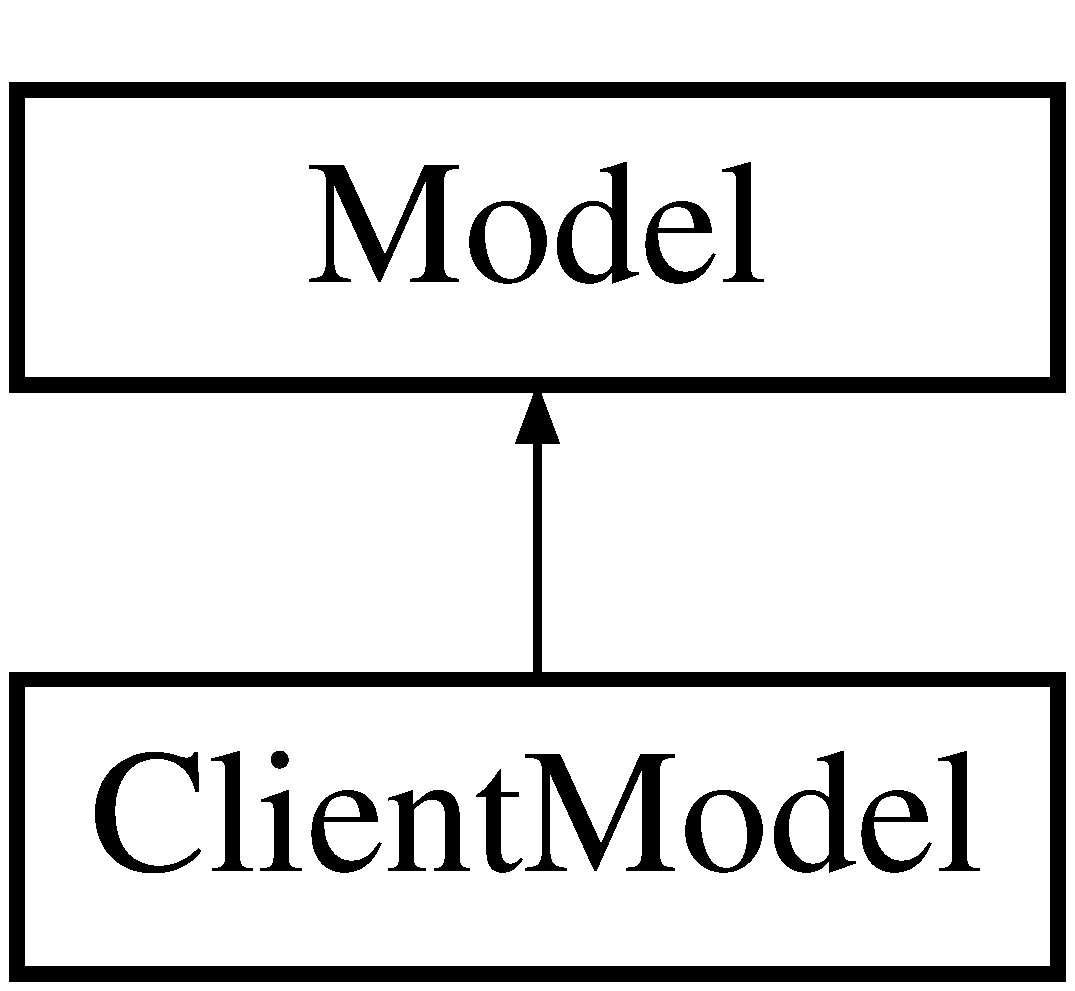
\includegraphics[height=2.000000cm]{classClientModel}
\end{center}
\end{figure}
\subsection*{Public Member Functions}
\begin{DoxyCompactItemize}
\item 
void \hyperlink{classClientModel_a7a843e039b6688f7c5252541ba712ef7}{render} ()
\item 
void \hyperlink{classClientModel_a437049cfcf845c836ad1f70305146daa}{show\-Board} ()
\item 
void \hyperlink{classClientModel_a0654ad96265273f41fb296bcf76ecca1}{show\-Players} ()
\item 
void \hyperlink{classClientModel_ae88e9b8273f5f81dfa7be9b8b0115c99}{update\-Board} (Rcf\-Client$<$ I\-\_\-\-Model $>$ \-\_\-client)
\item 
void \hyperlink{classClientModel_a05020d4d1665fea6f20f9ff633467cac}{update\-Players} (Rcf\-Client$<$ I\-\_\-\-Model $>$ \-\_\-client)
\item 
\hypertarget{classClientModel_a12044fc4df03e7651117c4cb0812810a}{void {\bfseries process} (Rcf\-Client$<$ I\-\_\-\-Model $>$ \-\_\-client)}\label{classClientModel_a12044fc4df03e7651117c4cb0812810a}

\end{DoxyCompactItemize}
\subsection*{Additional Inherited Members}


\subsection{Detailed Description}
Klasa modelu klienta 

\subsection{Member Function Documentation}
\hypertarget{classClientModel_a7a843e039b6688f7c5252541ba712ef7}{\index{Client\-Model@{Client\-Model}!render@{render}}
\index{render@{render}!ClientModel@{Client\-Model}}
\subsubsection[{render}]{\setlength{\rightskip}{0pt plus 5cm}void Client\-Model\-::render (
\begin{DoxyParamCaption}
{}
\end{DoxyParamCaption}
)\hspace{0.3cm}{\ttfamily [inline]}}}\label{classClientModel_a7a843e039b6688f7c5252541ba712ef7}
Funkcja renderujaca cala aplikacje. \hypertarget{classClientModel_a437049cfcf845c836ad1f70305146daa}{\index{Client\-Model@{Client\-Model}!show\-Board@{show\-Board}}
\index{show\-Board@{show\-Board}!ClientModel@{Client\-Model}}
\subsubsection[{show\-Board}]{\setlength{\rightskip}{0pt plus 5cm}void Client\-Model\-::show\-Board (
\begin{DoxyParamCaption}
{}
\end{DoxyParamCaption}
)\hspace{0.3cm}{\ttfamily [inline]}}}\label{classClientModel_a437049cfcf845c836ad1f70305146daa}
Wyswietla plansze. \hypertarget{classClientModel_a0654ad96265273f41fb296bcf76ecca1}{\index{Client\-Model@{Client\-Model}!show\-Players@{show\-Players}}
\index{show\-Players@{show\-Players}!ClientModel@{Client\-Model}}
\subsubsection[{show\-Players}]{\setlength{\rightskip}{0pt plus 5cm}void Client\-Model\-::show\-Players (
\begin{DoxyParamCaption}
{}
\end{DoxyParamCaption}
)\hspace{0.3cm}{\ttfamily [inline]}}}\label{classClientModel_a0654ad96265273f41fb296bcf76ecca1}
Wyswietla liste graczy. \hypertarget{classClientModel_ae88e9b8273f5f81dfa7be9b8b0115c99}{\index{Client\-Model@{Client\-Model}!update\-Board@{update\-Board}}
\index{update\-Board@{update\-Board}!ClientModel@{Client\-Model}}
\subsubsection[{update\-Board}]{\setlength{\rightskip}{0pt plus 5cm}void Client\-Model\-::update\-Board (
\begin{DoxyParamCaption}
\item[{Rcf\-Client$<$ I\-\_\-\-Model $>$}]{\-\_\-client}
\end{DoxyParamCaption}
)\hspace{0.3cm}{\ttfamily [inline]}}}\label{classClientModel_ae88e9b8273f5f81dfa7be9b8b0115c99}
Pobiera aktualny stan planszy z serwera. \hypertarget{classClientModel_a05020d4d1665fea6f20f9ff633467cac}{\index{Client\-Model@{Client\-Model}!update\-Players@{update\-Players}}
\index{update\-Players@{update\-Players}!ClientModel@{Client\-Model}}
\subsubsection[{update\-Players}]{\setlength{\rightskip}{0pt plus 5cm}void Client\-Model\-::update\-Players (
\begin{DoxyParamCaption}
\item[{Rcf\-Client$<$ I\-\_\-\-Model $>$}]{\-\_\-client}
\end{DoxyParamCaption}
)\hspace{0.3cm}{\ttfamily [inline]}}}\label{classClientModel_a05020d4d1665fea6f20f9ff633467cac}
Pobiera aktualna liste graczy. 

The documentation for this class was generated from the following file\-:\begin{DoxyCompactItemize}
\item 
Client.\-cpp\end{DoxyCompactItemize}

\hypertarget{classModel}{\section{Model Class Reference}
\label{classModel}\index{Model@{Model}}
}
Inheritance diagram for Model\-:\begin{figure}[H]
\begin{center}
\leavevmode
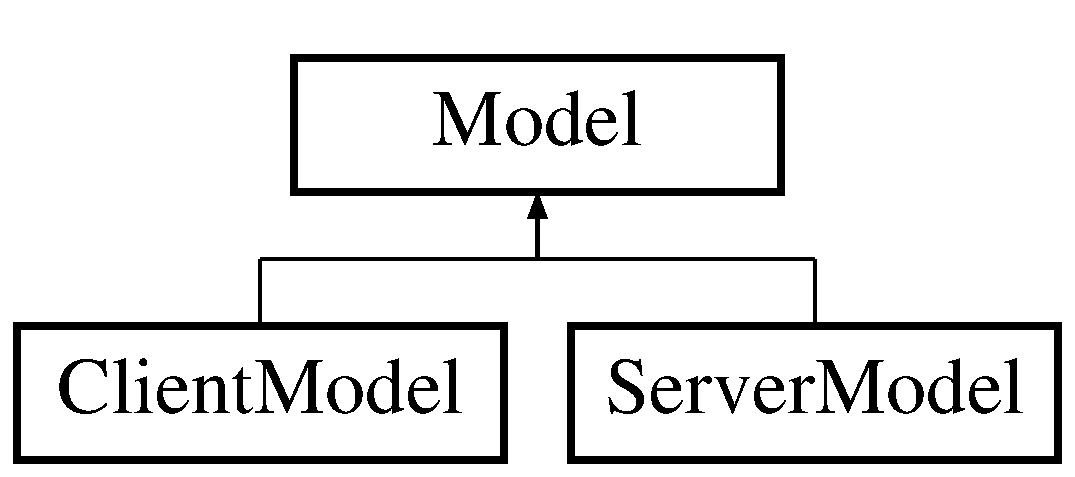
\includegraphics[height=2.000000cm]{classModel}
\end{center}
\end{figure}
\subsection*{Public Attributes}
\begin{DoxyCompactItemize}
\item 
int \hyperlink{classModel_a944736812928acb65055f5c7229970ae}{size}
\item 
int \hyperlink{classModel_a882710d0512c34c6b9b385c8d76825cb}{currplayer}
\item 
int \hyperlink{classModel_aa90bb7e95e18111d59df116fcabbdd89}{maxplayers}
\item 
int \hyperlink{classModel_addac0dda85cc75450345d300c48ff276}{idcounter}
\item 
bool \hyperlink{classModel_a46db7d7d8e79bf0bebd19c3e0122fba0}{running}
\item 
\hypertarget{classModel_a9e938f44d01e9e872152b1cad3f81646}{vector$<$ vector$<$ \hyperlink{classBlock}{Block} $>$ $>$ {\bfseries board}}\label{classModel_a9e938f44d01e9e872152b1cad3f81646}

\item 
vector$<$ \hyperlink{classPosition}{Position} $>$ \hyperlink{classModel_a082090abc6b22e3bb5354f892417c444}{free\-Tiles}
\item 
vector$<$ \hyperlink{classPlayer}{Player} $>$ \hyperlink{classModel_ae426f6b24893143e51e626a3026938ec}{players}
\item 
vector$<$ \hyperlink{classPlayer}{Player} $>$ \hyperlink{classModel_a268ae9f01416e04638a2424ee0e457ac}{spectators}
\end{DoxyCompactItemize}


\subsection{Detailed Description}
Klasa glowna modelu 

\subsection{Member Data Documentation}
\hypertarget{classModel_a882710d0512c34c6b9b385c8d76825cb}{\index{Model@{Model}!currplayer@{currplayer}}
\index{currplayer@{currplayer}!Model@{Model}}
\subsubsection[{currplayer}]{\setlength{\rightskip}{0pt plus 5cm}int Model\-::currplayer}}\label{classModel_a882710d0512c34c6b9b385c8d76825cb}
Aktualny gracz ktory ma ture \hypertarget{classModel_a082090abc6b22e3bb5354f892417c444}{\index{Model@{Model}!free\-Tiles@{free\-Tiles}}
\index{free\-Tiles@{free\-Tiles}!Model@{Model}}
\subsubsection[{free\-Tiles}]{\setlength{\rightskip}{0pt plus 5cm}vector$<$ {\bf Position} $>$ Model\-::free\-Tiles}}\label{classModel_a082090abc6b22e3bb5354f892417c444}
Plansza \hypertarget{classModel_addac0dda85cc75450345d300c48ff276}{\index{Model@{Model}!idcounter@{idcounter}}
\index{idcounter@{idcounter}!Model@{Model}}
\subsubsection[{idcounter}]{\setlength{\rightskip}{0pt plus 5cm}int Model\-::idcounter}}\label{classModel_addac0dda85cc75450345d300c48ff276}
Zmienna z ktorej przydzielane sa id dla graczy \hypertarget{classModel_aa90bb7e95e18111d59df116fcabbdd89}{\index{Model@{Model}!maxplayers@{maxplayers}}
\index{maxplayers@{maxplayers}!Model@{Model}}
\subsubsection[{maxplayers}]{\setlength{\rightskip}{0pt plus 5cm}int Model\-::maxplayers}}\label{classModel_aa90bb7e95e18111d59df116fcabbdd89}
Maksymalna ilosc graczy \hypertarget{classModel_ae426f6b24893143e51e626a3026938ec}{\index{Model@{Model}!players@{players}}
\index{players@{players}!Model@{Model}}
\subsubsection[{players}]{\setlength{\rightskip}{0pt plus 5cm}vector$<$ {\bf Player} $>$ Model\-::players}}\label{classModel_ae426f6b24893143e51e626a3026938ec}
Wolne pola na planszy \hypertarget{classModel_a46db7d7d8e79bf0bebd19c3e0122fba0}{\index{Model@{Model}!running@{running}}
\index{running@{running}!Model@{Model}}
\subsubsection[{running}]{\setlength{\rightskip}{0pt plus 5cm}bool Model\-::running}}\label{classModel_a46db7d7d8e79bf0bebd19c3e0122fba0}
Flaga oznaczajaca przebieg rozgrywki \hypertarget{classModel_a944736812928acb65055f5c7229970ae}{\index{Model@{Model}!size@{size}}
\index{size@{size}!Model@{Model}}
\subsubsection[{size}]{\setlength{\rightskip}{0pt plus 5cm}int Model\-::size}}\label{classModel_a944736812928acb65055f5c7229970ae}
Wielkosc planszy \hypertarget{classModel_a268ae9f01416e04638a2424ee0e457ac}{\index{Model@{Model}!spectators@{spectators}}
\index{spectators@{spectators}!Model@{Model}}
\subsubsection[{spectators}]{\setlength{\rightskip}{0pt plus 5cm}vector$<$ {\bf Player} $>$ Model\-::spectators}}\label{classModel_a268ae9f01416e04638a2424ee0e457ac}
Lista graczy 

The documentation for this class was generated from the following files\-:\begin{DoxyCompactItemize}
\item 
Client.\-cpp\item 
Server.\-cpp\end{DoxyCompactItemize}

\hypertarget{classPlayer}{\section{Player Class Reference}
\label{classPlayer}\index{Player@{Player}}
}
\subsection*{Public Member Functions}
\begin{DoxyCompactItemize}
\item 
\hypertarget{classPlayer_a7e73d9e077fb15be7af8baf6e8924d6c}{{\bfseries Player} (string \-\_\-nick, int \-\_\-score, int \-\_\-wins)}\label{classPlayer_a7e73d9e077fb15be7af8baf6e8924d6c}

\item 
\hypertarget{classPlayer_aae48749805799debc558ad74c2cfbc8d}{void {\bfseries set\-Id} (int val)}\label{classPlayer_aae48749805799debc558ad74c2cfbc8d}

\item 
\hypertarget{classPlayer_aa206440e032fa4a2ff1ea4ebf7814897}{{\bfseries Player} (string \-\_\-nick)}\label{classPlayer_aa206440e032fa4a2ff1ea4ebf7814897}

\item 
\hypertarget{classPlayer_aae48749805799debc558ad74c2cfbc8d}{void {\bfseries set\-Id} (int val)}\label{classPlayer_aae48749805799debc558ad74c2cfbc8d}

\end{DoxyCompactItemize}
\subsection*{Public Attributes}
\begin{DoxyCompactItemize}
\item 
int \hyperlink{classPlayer_a05e05f3a23de78da7ec032ec2bcf8c6c}{id}
\item 
string \hyperlink{classPlayer_aea2f8abddadf8deb423a3c9b507d1ccc}{nick}
\item 
int \hyperlink{classPlayer_ace6abae8d66534ad0a1fd6458f786a6e}{score}
\item 
int \hyperlink{classPlayer_aba7987685c25a4189ae664e9748eecf0}{wins}
\item 
bool \hyperlink{classPlayer_a8039b9f17594c036c3bd7b676a24b19e}{empty}
\item 
bool \hyperlink{classPlayer_a1b72316124caf757250c3cee1c4416ff}{check}
\end{DoxyCompactItemize}


\subsection{Detailed Description}
Klasa gracza 

\subsection{Member Data Documentation}
\hypertarget{classPlayer_a1b72316124caf757250c3cee1c4416ff}{\index{Player@{Player}!check@{check}}
\index{check@{check}!Player@{Player}}
\subsubsection[{check}]{\setlength{\rightskip}{0pt plus 5cm}bool Player\-::check}}\label{classPlayer_a1b72316124caf757250c3cee1c4416ff}
Czy gracz sie odmeldowal na serwerze \hypertarget{classPlayer_a8039b9f17594c036c3bd7b676a24b19e}{\index{Player@{Player}!empty@{empty}}
\index{empty@{empty}!Player@{Player}}
\subsubsection[{empty}]{\setlength{\rightskip}{0pt plus 5cm}bool Player\-::empty}}\label{classPlayer_a8039b9f17594c036c3bd7b676a24b19e}
Czy gracz jest aktywny \hypertarget{classPlayer_a05e05f3a23de78da7ec032ec2bcf8c6c}{\index{Player@{Player}!id@{id}}
\index{id@{id}!Player@{Player}}
\subsubsection[{id}]{\setlength{\rightskip}{0pt plus 5cm}int Player\-::id}}\label{classPlayer_a05e05f3a23de78da7ec032ec2bcf8c6c}
I\-D gracza \hypertarget{classPlayer_aea2f8abddadf8deb423a3c9b507d1ccc}{\index{Player@{Player}!nick@{nick}}
\index{nick@{nick}!Player@{Player}}
\subsubsection[{nick}]{\setlength{\rightskip}{0pt plus 5cm}string Player\-::nick}}\label{classPlayer_aea2f8abddadf8deb423a3c9b507d1ccc}
Nick gracza \hypertarget{classPlayer_ace6abae8d66534ad0a1fd6458f786a6e}{\index{Player@{Player}!score@{score}}
\index{score@{score}!Player@{Player}}
\subsubsection[{score}]{\setlength{\rightskip}{0pt plus 5cm}int Player\-::score}}\label{classPlayer_ace6abae8d66534ad0a1fd6458f786a6e}
Aktualny wynik gracza \hypertarget{classPlayer_aba7987685c25a4189ae664e9748eecf0}{\index{Player@{Player}!wins@{wins}}
\index{wins@{wins}!Player@{Player}}
\subsubsection[{wins}]{\setlength{\rightskip}{0pt plus 5cm}int Player\-::wins}}\label{classPlayer_aba7987685c25a4189ae664e9748eecf0}
Ilosc zwyciestw 

The documentation for this class was generated from the following files\-:\begin{DoxyCompactItemize}
\item 
Client.\-cpp\item 
Server.\-cpp\end{DoxyCompactItemize}

\hypertarget{classPosition}{\section{Position Class Reference}
\label{classPosition}\index{Position@{Position}}
}
\subsection*{Public Member Functions}
\begin{DoxyCompactItemize}
\item 
\hypertarget{classPosition_a6e36cf0fee251e74cfedb86f4e99558d}{{\bfseries Position} (int x, int y)}\label{classPosition_a6e36cf0fee251e74cfedb86f4e99558d}

\item 
\hypertarget{classPosition_a6e36cf0fee251e74cfedb86f4e99558d}{{\bfseries Position} (int x, int y)}\label{classPosition_a6e36cf0fee251e74cfedb86f4e99558d}

\item 
\hypertarget{classPosition_a6e36cf0fee251e74cfedb86f4e99558d}{{\bfseries Position} (int x, int y)}\label{classPosition_a6e36cf0fee251e74cfedb86f4e99558d}

\end{DoxyCompactItemize}
\subsection*{Public Attributes}
\begin{DoxyCompactItemize}
\item 
\hypertarget{classPosition_aeda152ffeee17ae5be9c02327b2408d8}{int {\bfseries x}}\label{classPosition_aeda152ffeee17ae5be9c02327b2408d8}

\item 
\hypertarget{classPosition_a3c08e9213d4726b21caba3073192c4a3}{int {\bfseries y}}\label{classPosition_a3c08e9213d4726b21caba3073192c4a3}

\end{DoxyCompactItemize}


\subsection{Detailed Description}
Klasa pomocnicza 

The documentation for this class was generated from the following files\-:\begin{DoxyCompactItemize}
\item 
board.\-cpp\item 
Client.\-cpp\item 
Server.\-cpp\end{DoxyCompactItemize}

\hypertarget{classServerModel}{\section{Server\-Model Class Reference}
\label{classServerModel}\index{Server\-Model@{Server\-Model}}
}
Inheritance diagram for Server\-Model\-:\begin{figure}[H]
\begin{center}
\leavevmode
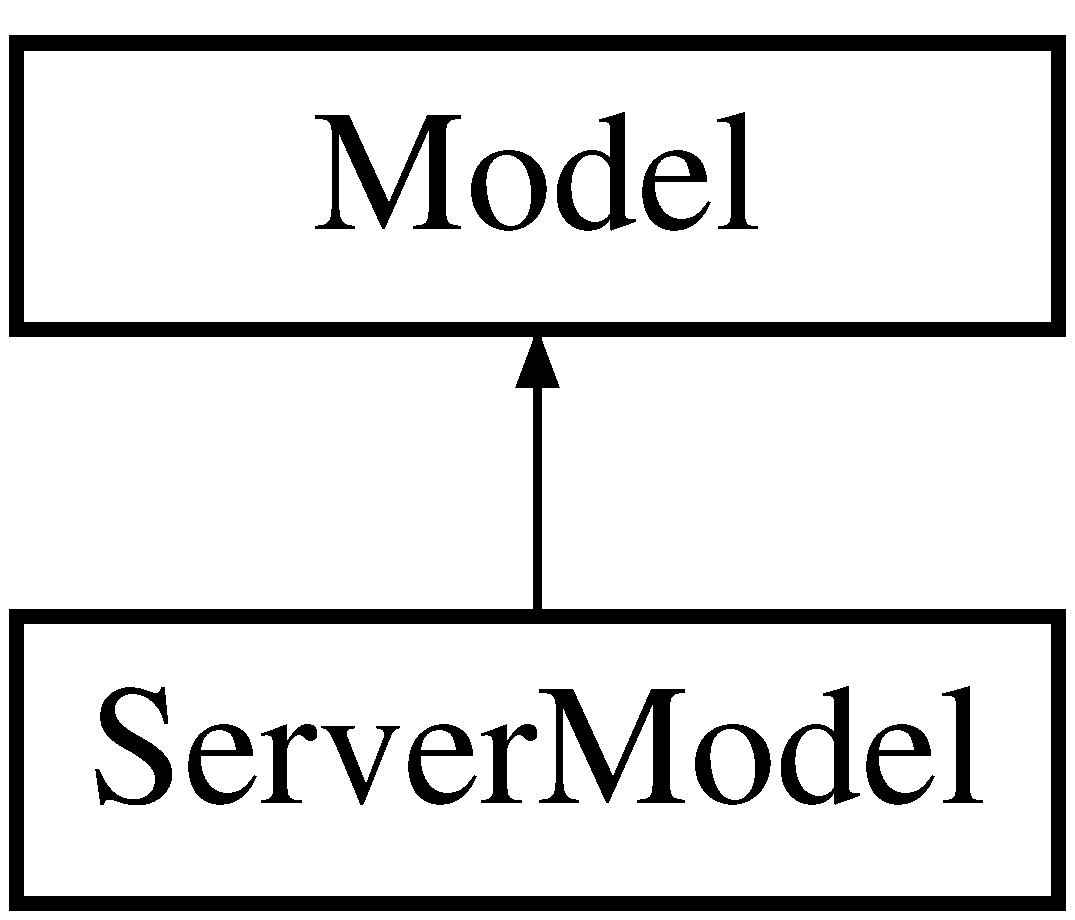
\includegraphics[height=2.000000cm]{classServerModel}
\end{center}
\end{figure}
\subsection*{Public Member Functions}
\begin{DoxyCompactItemize}
\item 
int \hyperlink{classServerModel_a8002df80f7319f9cc726ecf6f1cb295e}{add\-Player} (const string \-\_\-nick)
\item 
void \hyperlink{classServerModel_a03636f686c14d807e5f8e7527b4f3eca}{remove\-Player} (const int \-\_\-id)
\item 
vector$<$ string $>$ \hyperlink{classServerModel_abd04bc42130f10b6fcf9f6ff96441fe7}{get\-Nicks} ()
\item 
vector$<$ int $>$ \hyperlink{classServerModel_a42da33b42e600dfe892509a3e1f04fb0}{get\-Scores} ()
\item 
int \hyperlink{classServerModel_a53887668e0e8193fb345710d76dd12b7}{get\-Player\-Count} ()
\item 
int \hyperlink{classServerModel_a02e91f06a02510759b370eefbcb52061}{get\-Curr\-Player} ()
\item 
void \hyperlink{classServerModel_af98c5669849c1d648b6103fda3f4a10c}{switch\-Player} ()
\item 
bool \hyperlink{classServerModel_ab4cf786672a46e6285eb72907005ae64}{check\-My\-Turn} (int \-\_\-id)
\item 
void \hyperlink{classServerModel_a5ccabb0400aff1109578dacfc1162af4}{reset} ()
\item 
void \hyperlink{classServerModel_a7b17b497feec14ba4ea7746f17b479e9}{reset\-Scores} ()
\item 
void \hyperlink{classServerModel_a277375b608707d6f6c308f4a8af2e1b7}{update\-Free\-Tiles} ()
\item 
void \hyperlink{classServerModel_ad3b7678f205acbf9a6efe65ba60cfd73}{clear\-Adv} ()
\item 
bool \hyperlink{classServerModel_a71bd99e883342592c9f9842c63503044}{move\-Up} ()
\item 
bool \hyperlink{classServerModel_ac12b01ceb25260cee42e4b2f6c5afa00}{move\-Down} ()
\item 
bool \hyperlink{classServerModel_a3d33c6ca6db221fb38b12ddcd1b973d7}{move\-Left} ()
\item 
bool \hyperlink{classServerModel_a12a3fcd85eda6068b85401f398ba567f}{move\-Right} ()
\item 
bool \hyperlink{classServerModel_addd72dd4e20c62633121da9e75907cf0}{check\-Occupy} ()
\item 
bool \hyperlink{classServerModel_acb1a12dd3af4d4ae84ce6a76742bc5b0}{check\-Move} ()
\item 
void \hyperlink{classServerModel_a0f9e52d858f03acff61df4ec297fbc87}{check\-End\-Game} ()
\item 
\hyperlink{classPlayer}{Player} \hyperlink{classServerModel_a7b23bfe191a3f618f260c781e5306e57}{get\-Winner} ()
\item 
bool \hyperlink{classServerModel_a2ed41cae52af16d5410b0669cce5fc7a}{move} (int dir)
\item 
void \hyperlink{classServerModel_a84fbe35ac950f1b71da800e14ac85814}{turn} (const int dir)
\item 
void \hyperlink{classServerModel_a30ce9865dba626f3aca22e6355d45a79}{rand\-Spawn} ()
\item 
void \hyperlink{classServerModel_a8f187ffda03256f2aa2679b22399d8ed}{showboard} ()
\item 
vector$<$ vector$<$ double $>$ $>$ \hyperlink{classServerModel_a0cdcac1cfe266b4fdaf9b0251a6f6553}{get\-Board} ()
\item 
void \hyperlink{classServerModel_a155230e9bb8373cfe4eaedbb87b05c0c}{check\-Player} (int \-\_\-id)
\item 
void \hyperlink{classServerModel_a402b44d30f2b3207154a67db4c28982f}{reset\-Checks} ()
\item 
void \hyperlink{classServerModel_aedccd8017caa1e8a9ed5a323d19d424e}{check\-Alive\-Players} ()
\end{DoxyCompactItemize}
\subsection*{Additional Inherited Members}


\subsection{Detailed Description}
Klasa modelu serwera 

\subsection{Member Function Documentation}
\hypertarget{classServerModel_a8002df80f7319f9cc726ecf6f1cb295e}{\index{Server\-Model@{Server\-Model}!add\-Player@{add\-Player}}
\index{add\-Player@{add\-Player}!ServerModel@{Server\-Model}}
\subsubsection[{add\-Player}]{\setlength{\rightskip}{0pt plus 5cm}int Server\-Model\-::add\-Player (
\begin{DoxyParamCaption}
\item[{const string}]{\-\_\-nick}
\end{DoxyParamCaption}
)\hspace{0.3cm}{\ttfamily [inline]}}}\label{classServerModel_a8002df80f7319f9cc726ecf6f1cb295e}
Dodaje gracza do gry z nickiem podanym w argumencie. Jesli nie ma miejsca to klient zostaje dodany jako widz. \hypertarget{classServerModel_aedccd8017caa1e8a9ed5a323d19d424e}{\index{Server\-Model@{Server\-Model}!check\-Alive\-Players@{check\-Alive\-Players}}
\index{check\-Alive\-Players@{check\-Alive\-Players}!ServerModel@{Server\-Model}}
\subsubsection[{check\-Alive\-Players}]{\setlength{\rightskip}{0pt plus 5cm}void Server\-Model\-::check\-Alive\-Players (
\begin{DoxyParamCaption}
{}
\end{DoxyParamCaption}
)\hspace{0.3cm}{\ttfamily [inline]}}}\label{classServerModel_aedccd8017caa1e8a9ed5a323d19d424e}
Detekcja martwych klientow. \hypertarget{classServerModel_a0f9e52d858f03acff61df4ec297fbc87}{\index{Server\-Model@{Server\-Model}!check\-End\-Game@{check\-End\-Game}}
\index{check\-End\-Game@{check\-End\-Game}!ServerModel@{Server\-Model}}
\subsubsection[{check\-End\-Game}]{\setlength{\rightskip}{0pt plus 5cm}void Server\-Model\-::check\-End\-Game (
\begin{DoxyParamCaption}
{}
\end{DoxyParamCaption}
)\hspace{0.3cm}{\ttfamily [inline]}}}\label{classServerModel_a0f9e52d858f03acff61df4ec297fbc87}
Sprawdza koniec gry. \hypertarget{classServerModel_acb1a12dd3af4d4ae84ce6a76742bc5b0}{\index{Server\-Model@{Server\-Model}!check\-Move@{check\-Move}}
\index{check\-Move@{check\-Move}!ServerModel@{Server\-Model}}
\subsubsection[{check\-Move}]{\setlength{\rightskip}{0pt plus 5cm}bool Server\-Model\-::check\-Move (
\begin{DoxyParamCaption}
{}
\end{DoxyParamCaption}
)\hspace{0.3cm}{\ttfamily [inline]}}}\label{classServerModel_acb1a12dd3af4d4ae84ce6a76742bc5b0}
Sprawdza mozliwosc ruchu. \hypertarget{classServerModel_ab4cf786672a46e6285eb72907005ae64}{\index{Server\-Model@{Server\-Model}!check\-My\-Turn@{check\-My\-Turn}}
\index{check\-My\-Turn@{check\-My\-Turn}!ServerModel@{Server\-Model}}
\subsubsection[{check\-My\-Turn}]{\setlength{\rightskip}{0pt plus 5cm}bool Server\-Model\-::check\-My\-Turn (
\begin{DoxyParamCaption}
\item[{int}]{\-\_\-id}
\end{DoxyParamCaption}
)\hspace{0.3cm}{\ttfamily [inline]}}}\label{classServerModel_ab4cf786672a46e6285eb72907005ae64}
Sprawdzenie czy gracz o podanym id aktualnie ma ture. \hypertarget{classServerModel_addd72dd4e20c62633121da9e75907cf0}{\index{Server\-Model@{Server\-Model}!check\-Occupy@{check\-Occupy}}
\index{check\-Occupy@{check\-Occupy}!ServerModel@{Server\-Model}}
\subsubsection[{check\-Occupy}]{\setlength{\rightskip}{0pt plus 5cm}bool Server\-Model\-::check\-Occupy (
\begin{DoxyParamCaption}
{}
\end{DoxyParamCaption}
)\hspace{0.3cm}{\ttfamily [inline]}}}\label{classServerModel_addd72dd4e20c62633121da9e75907cf0}
Sprawdzenie czy nie ma wolnych pol na planszy. \hypertarget{classServerModel_a155230e9bb8373cfe4eaedbb87b05c0c}{\index{Server\-Model@{Server\-Model}!check\-Player@{check\-Player}}
\index{check\-Player@{check\-Player}!ServerModel@{Server\-Model}}
\subsubsection[{check\-Player}]{\setlength{\rightskip}{0pt plus 5cm}void Server\-Model\-::check\-Player (
\begin{DoxyParamCaption}
\item[{int}]{\-\_\-id}
\end{DoxyParamCaption}
)\hspace{0.3cm}{\ttfamily [inline]}}}\label{classServerModel_a155230e9bb8373cfe4eaedbb87b05c0c}
Sprawdzenie listy obecnosci. \hypertarget{classServerModel_ad3b7678f205acbf9a6efe65ba60cfd73}{\index{Server\-Model@{Server\-Model}!clear\-Adv@{clear\-Adv}}
\index{clear\-Adv@{clear\-Adv}!ServerModel@{Server\-Model}}
\subsubsection[{clear\-Adv}]{\setlength{\rightskip}{0pt plus 5cm}void Server\-Model\-::clear\-Adv (
\begin{DoxyParamCaption}
{}
\end{DoxyParamCaption}
)\hspace{0.3cm}{\ttfamily [inline]}}}\label{classServerModel_ad3b7678f205acbf9a6efe65ba60cfd73}
Czyszczenie pol adv na calej planszy. \hypertarget{classServerModel_a0cdcac1cfe266b4fdaf9b0251a6f6553}{\index{Server\-Model@{Server\-Model}!get\-Board@{get\-Board}}
\index{get\-Board@{get\-Board}!ServerModel@{Server\-Model}}
\subsubsection[{get\-Board}]{\setlength{\rightskip}{0pt plus 5cm}vector$<$ vector$<$double$>$ $>$ Server\-Model\-::get\-Board (
\begin{DoxyParamCaption}
{}
\end{DoxyParamCaption}
)\hspace{0.3cm}{\ttfamily [inline]}}}\label{classServerModel_a0cdcac1cfe266b4fdaf9b0251a6f6553}
Zwraca plansze. \hypertarget{classServerModel_a02e91f06a02510759b370eefbcb52061}{\index{Server\-Model@{Server\-Model}!get\-Curr\-Player@{get\-Curr\-Player}}
\index{get\-Curr\-Player@{get\-Curr\-Player}!ServerModel@{Server\-Model}}
\subsubsection[{get\-Curr\-Player}]{\setlength{\rightskip}{0pt plus 5cm}int Server\-Model\-::get\-Curr\-Player (
\begin{DoxyParamCaption}
{}
\end{DoxyParamCaption}
)\hspace{0.3cm}{\ttfamily [inline]}}}\label{classServerModel_a02e91f06a02510759b370eefbcb52061}
Zwraca numer gracza, ktory ma ture. \hypertarget{classServerModel_abd04bc42130f10b6fcf9f6ff96441fe7}{\index{Server\-Model@{Server\-Model}!get\-Nicks@{get\-Nicks}}
\index{get\-Nicks@{get\-Nicks}!ServerModel@{Server\-Model}}
\subsubsection[{get\-Nicks}]{\setlength{\rightskip}{0pt plus 5cm}vector$<$string$>$ Server\-Model\-::get\-Nicks (
\begin{DoxyParamCaption}
{}
\end{DoxyParamCaption}
)\hspace{0.3cm}{\ttfamily [inline]}}}\label{classServerModel_abd04bc42130f10b6fcf9f6ff96441fe7}
Zwraca nicki aktualnie grajacych graczy. \hypertarget{classServerModel_a53887668e0e8193fb345710d76dd12b7}{\index{Server\-Model@{Server\-Model}!get\-Player\-Count@{get\-Player\-Count}}
\index{get\-Player\-Count@{get\-Player\-Count}!ServerModel@{Server\-Model}}
\subsubsection[{get\-Player\-Count}]{\setlength{\rightskip}{0pt plus 5cm}int Server\-Model\-::get\-Player\-Count (
\begin{DoxyParamCaption}
{}
\end{DoxyParamCaption}
)\hspace{0.3cm}{\ttfamily [inline]}}}\label{classServerModel_a53887668e0e8193fb345710d76dd12b7}
Zwraca ilosc grajacych. \hypertarget{classServerModel_a42da33b42e600dfe892509a3e1f04fb0}{\index{Server\-Model@{Server\-Model}!get\-Scores@{get\-Scores}}
\index{get\-Scores@{get\-Scores}!ServerModel@{Server\-Model}}
\subsubsection[{get\-Scores}]{\setlength{\rightskip}{0pt plus 5cm}vector$<$int$>$ Server\-Model\-::get\-Scores (
\begin{DoxyParamCaption}
{}
\end{DoxyParamCaption}
)\hspace{0.3cm}{\ttfamily [inline]}}}\label{classServerModel_a42da33b42e600dfe892509a3e1f04fb0}
Zwraca wyniki aktualnie grajacych graczy. \hypertarget{classServerModel_a7b23bfe191a3f618f260c781e5306e57}{\index{Server\-Model@{Server\-Model}!get\-Winner@{get\-Winner}}
\index{get\-Winner@{get\-Winner}!ServerModel@{Server\-Model}}
\subsubsection[{get\-Winner}]{\setlength{\rightskip}{0pt plus 5cm}{\bf Player} Server\-Model\-::get\-Winner (
\begin{DoxyParamCaption}
{}
\end{DoxyParamCaption}
)\hspace{0.3cm}{\ttfamily [inline]}}}\label{classServerModel_a7b23bfe191a3f618f260c781e5306e57}
Zwraca gracza zwyciezce. \hypertarget{classServerModel_a2ed41cae52af16d5410b0669cce5fc7a}{\index{Server\-Model@{Server\-Model}!move@{move}}
\index{move@{move}!ServerModel@{Server\-Model}}
\subsubsection[{move}]{\setlength{\rightskip}{0pt plus 5cm}bool Server\-Model\-::move (
\begin{DoxyParamCaption}
\item[{int}]{dir}
\end{DoxyParamCaption}
)\hspace{0.3cm}{\ttfamily [inline]}}}\label{classServerModel_a2ed41cae52af16d5410b0669cce5fc7a}
Ogolna funkcja obslugujaca ruch. \hypertarget{classServerModel_ac12b01ceb25260cee42e4b2f6c5afa00}{\index{Server\-Model@{Server\-Model}!move\-Down@{move\-Down}}
\index{move\-Down@{move\-Down}!ServerModel@{Server\-Model}}
\subsubsection[{move\-Down}]{\setlength{\rightskip}{0pt plus 5cm}bool Server\-Model\-::move\-Down (
\begin{DoxyParamCaption}
{}
\end{DoxyParamCaption}
)\hspace{0.3cm}{\ttfamily [inline]}}}\label{classServerModel_ac12b01ceb25260cee42e4b2f6c5afa00}
Ruch w dol. Zwraca czy nastapil ruch. \hypertarget{classServerModel_a3d33c6ca6db221fb38b12ddcd1b973d7}{\index{Server\-Model@{Server\-Model}!move\-Left@{move\-Left}}
\index{move\-Left@{move\-Left}!ServerModel@{Server\-Model}}
\subsubsection[{move\-Left}]{\setlength{\rightskip}{0pt plus 5cm}bool Server\-Model\-::move\-Left (
\begin{DoxyParamCaption}
{}
\end{DoxyParamCaption}
)\hspace{0.3cm}{\ttfamily [inline]}}}\label{classServerModel_a3d33c6ca6db221fb38b12ddcd1b973d7}
Ruch w lewo. Zwraca czy nastapil ruch. \hypertarget{classServerModel_a12a3fcd85eda6068b85401f398ba567f}{\index{Server\-Model@{Server\-Model}!move\-Right@{move\-Right}}
\index{move\-Right@{move\-Right}!ServerModel@{Server\-Model}}
\subsubsection[{move\-Right}]{\setlength{\rightskip}{0pt plus 5cm}bool Server\-Model\-::move\-Right (
\begin{DoxyParamCaption}
{}
\end{DoxyParamCaption}
)\hspace{0.3cm}{\ttfamily [inline]}}}\label{classServerModel_a12a3fcd85eda6068b85401f398ba567f}
Ruch w prawo. Zwraca czy nastapil ruch. \hypertarget{classServerModel_a71bd99e883342592c9f9842c63503044}{\index{Server\-Model@{Server\-Model}!move\-Up@{move\-Up}}
\index{move\-Up@{move\-Up}!ServerModel@{Server\-Model}}
\subsubsection[{move\-Up}]{\setlength{\rightskip}{0pt plus 5cm}bool Server\-Model\-::move\-Up (
\begin{DoxyParamCaption}
{}
\end{DoxyParamCaption}
)\hspace{0.3cm}{\ttfamily [inline]}}}\label{classServerModel_a71bd99e883342592c9f9842c63503044}
Ruch w gore. Zwraca czy nastapil ruch. \hypertarget{classServerModel_a30ce9865dba626f3aca22e6355d45a79}{\index{Server\-Model@{Server\-Model}!rand\-Spawn@{rand\-Spawn}}
\index{rand\-Spawn@{rand\-Spawn}!ServerModel@{Server\-Model}}
\subsubsection[{rand\-Spawn}]{\setlength{\rightskip}{0pt plus 5cm}void Server\-Model\-::rand\-Spawn (
\begin{DoxyParamCaption}
{}
\end{DoxyParamCaption}
)\hspace{0.3cm}{\ttfamily [inline]}}}\label{classServerModel_a30ce9865dba626f3aca22e6355d45a79}
Losowanie nowego numeru na planszy. \hypertarget{classServerModel_a03636f686c14d807e5f8e7527b4f3eca}{\index{Server\-Model@{Server\-Model}!remove\-Player@{remove\-Player}}
\index{remove\-Player@{remove\-Player}!ServerModel@{Server\-Model}}
\subsubsection[{remove\-Player}]{\setlength{\rightskip}{0pt plus 5cm}void Server\-Model\-::remove\-Player (
\begin{DoxyParamCaption}
\item[{const int}]{\-\_\-id}
\end{DoxyParamCaption}
)\hspace{0.3cm}{\ttfamily [inline]}}}\label{classServerModel_a03636f686c14d807e5f8e7527b4f3eca}
Usuwa gracza o podanym id. \hypertarget{classServerModel_a5ccabb0400aff1109578dacfc1162af4}{\index{Server\-Model@{Server\-Model}!reset@{reset}}
\index{reset@{reset}!ServerModel@{Server\-Model}}
\subsubsection[{reset}]{\setlength{\rightskip}{0pt plus 5cm}void Server\-Model\-::reset (
\begin{DoxyParamCaption}
{}
\end{DoxyParamCaption}
)\hspace{0.3cm}{\ttfamily [inline]}}}\label{classServerModel_a5ccabb0400aff1109578dacfc1162af4}
Reset planszy. \hypertarget{classServerModel_a402b44d30f2b3207154a67db4c28982f}{\index{Server\-Model@{Server\-Model}!reset\-Checks@{reset\-Checks}}
\index{reset\-Checks@{reset\-Checks}!ServerModel@{Server\-Model}}
\subsubsection[{reset\-Checks}]{\setlength{\rightskip}{0pt plus 5cm}void Server\-Model\-::reset\-Checks (
\begin{DoxyParamCaption}
{}
\end{DoxyParamCaption}
)\hspace{0.3cm}{\ttfamily [inline]}}}\label{classServerModel_a402b44d30f2b3207154a67db4c28982f}
Reset listy obecnosci. \hypertarget{classServerModel_a7b17b497feec14ba4ea7746f17b479e9}{\index{Server\-Model@{Server\-Model}!reset\-Scores@{reset\-Scores}}
\index{reset\-Scores@{reset\-Scores}!ServerModel@{Server\-Model}}
\subsubsection[{reset\-Scores}]{\setlength{\rightskip}{0pt plus 5cm}void Server\-Model\-::reset\-Scores (
\begin{DoxyParamCaption}
{}
\end{DoxyParamCaption}
)\hspace{0.3cm}{\ttfamily [inline]}}}\label{classServerModel_a7b17b497feec14ba4ea7746f17b479e9}
Reset wyników. \hypertarget{classServerModel_a8f187ffda03256f2aa2679b22399d8ed}{\index{Server\-Model@{Server\-Model}!showboard@{showboard}}
\index{showboard@{showboard}!ServerModel@{Server\-Model}}
\subsubsection[{showboard}]{\setlength{\rightskip}{0pt plus 5cm}void Server\-Model\-::showboard (
\begin{DoxyParamCaption}
{}
\end{DoxyParamCaption}
)\hspace{0.3cm}{\ttfamily [inline]}}}\label{classServerModel_a8f187ffda03256f2aa2679b22399d8ed}
Wyswietla plansze. \hypertarget{classServerModel_af98c5669849c1d648b6103fda3f4a10c}{\index{Server\-Model@{Server\-Model}!switch\-Player@{switch\-Player}}
\index{switch\-Player@{switch\-Player}!ServerModel@{Server\-Model}}
\subsubsection[{switch\-Player}]{\setlength{\rightskip}{0pt plus 5cm}void Server\-Model\-::switch\-Player (
\begin{DoxyParamCaption}
{}
\end{DoxyParamCaption}
)\hspace{0.3cm}{\ttfamily [inline]}}}\label{classServerModel_af98c5669849c1d648b6103fda3f4a10c}
Przelaczenie tury na nastepnego gracza. \hypertarget{classServerModel_a84fbe35ac950f1b71da800e14ac85814}{\index{Server\-Model@{Server\-Model}!turn@{turn}}
\index{turn@{turn}!ServerModel@{Server\-Model}}
\subsubsection[{turn}]{\setlength{\rightskip}{0pt plus 5cm}void Server\-Model\-::turn (
\begin{DoxyParamCaption}
\item[{const int}]{dir}
\end{DoxyParamCaption}
)\hspace{0.3cm}{\ttfamily [inline]}}}\label{classServerModel_a84fbe35ac950f1b71da800e14ac85814}
Wykonanie tury. \hypertarget{classServerModel_a277375b608707d6f6c308f4a8af2e1b7}{\index{Server\-Model@{Server\-Model}!update\-Free\-Tiles@{update\-Free\-Tiles}}
\index{update\-Free\-Tiles@{update\-Free\-Tiles}!ServerModel@{Server\-Model}}
\subsubsection[{update\-Free\-Tiles}]{\setlength{\rightskip}{0pt plus 5cm}void Server\-Model\-::update\-Free\-Tiles (
\begin{DoxyParamCaption}
{}
\end{DoxyParamCaption}
)\hspace{0.3cm}{\ttfamily [inline]}}}\label{classServerModel_a277375b608707d6f6c308f4a8af2e1b7}
Aktualizacja wolnych pol. 

The documentation for this class was generated from the following file\-:\begin{DoxyCompactItemize}
\item 
Server.\-cpp\end{DoxyCompactItemize}

%--- End generated contents ---

% Index
\newpage
\phantomsection
\addcontentsline{toc}{chapter}{Index}
\printindex

\end{document}
